% https://topanswers.xyz/tex?q=1244#a1476
\documentclass{beamer}
\beamertemplatenavigationsymbolsempty
\setbeamertemplate{frametitle}[default][center]
\usepackage[many]{tcolorbox}
\usepackage{listings}
\lstdefinestyle{duckstyle}{%
    moredelim=[is][\color{red}]{|}{|},
    mathescape=true,
    escapechar=@,
    basicstyle=\ttfamily,
    columns=fullflexible
}
\lstset{style=duckstyle}
\newcommand{\ubar}[1]{\alt<+>{\underaccent{\bar}{#1}}{#1}}
\tcbuselibrary{skins}
\tcbset{
	arc=0pt,
	outer arc=0pt,
	colback=white,
}
\usepackage{tikz}
\usetikzlibrary{arrows.meta,
	shapes,
	tikzmark}
\usetikzlibrary{tikzmark,shapes.geometric}
\usetikzmarklibrary{listings} 

\usepackage{calc}

\newcommand{\Proc}[1]{\textsc{#1}}
\newcommand{\Var}[1]{\ensuremath{\textcolor{varcolor}{#1}}}
\definecolor{varcolor}{RGB}{15,122,183}

\makeatletter
\gdef\lst@SetFirstNumber{%
    \ifx\lst@firstnumber\@undefined
%        \@tempcnta 0\csname\@lst no@\lst@intname\endcsname\relax
        \@tempcnta=1%
        \ifnum\@tempcnta=\z@ \else
            \lst@nololtrue
            \advance\@tempcnta\lst@advancenumber
            \edef\lst@firstnumber{\the\@tempcnta\relax}%
        \fi
    \fi}%
\makeatother


\definecolor{titlecolor}{RGB}{29, 110, 174}
\begin{document}
\begin{frame}[t, fragile]{}
Some text written here introducing the slide to the spectators.
\begin{columns}

\begin{column}{5.2cm} %

    \begin{tcolorbox}[top=0pt, left=5pt,right=5pt, colback=blue!5!white, text width=5.2cm, text height=7cm]
\begin{lstlisting}[mathescape, name=misra, basewidth = {.3em}]
Algorithm($\Var{a_1,a_2,\dots,a_m}$)

set $\Var{A}$ = $\emptyset$
\end{lstlisting}
\end{tcolorbox}
\end{column}
    
   
\begin{column}{\textwidth-5cm} %
\vspace{-0.8cm}
\begin{center}
\begin{tcolorbox}[top=0pt, left=5pt,right=5pt, colframe=blue, text width=4cm, text height=0.8cm]
\end{tcolorbox}
\end{center}
\begin{itemize}[<+->] 
\setlength\itemsep{5pt plus 1fill}
\item[] $\tikzmark{step1}A \rightarrow \tilde{f}_A = 1 $
\item[] $C \rightarrow \tilde{f}_A = 1, \tilde{f}_C = 1$
\end{itemize}

\end{column}
    \begin{tikzpicture}[remember picture]
    \draw[->,overlay, dashed] (pic cs:step1) to [bend right]([xshift=0.2cm, yshift=.25\baselineskip]pic cs:line-misra-3-end);
    \end{tikzpicture}
\end{columns}
\end{frame}


\end{document}